\chapter{Controllo $H_\infty$: baseline e revisione controllata}
\label{cap:hinf}
\section{Obiettivo, perimetro e baseline conservata}
Questa revisione riguarda esclusivamente M9--M11. Pianta M3, modello
incerto M4, specifiche generali M5, LQG/LQRI, Kalman e RAS M6--M8
rimangono congelati. Tutti i precedenti artifact M9/M10/M11 sono conservati
integralmente; i nuovi risultati sono in una directory separata.
Il Capitolo 9 e i successivi descrivono la catena storica e non certificano
i controllori qui introdotti. Anche il riepilogo generale precedente
resta riferito alla baseline, in attesa della revisione successiva autorizzata.

La traccia consente semplificazioni motivate delle prestazioni.
I due gradi di liberta' indicano i due giunti del manipolatore, non impongono
un'architettura di controllo a due gradi di liberta'. La sintesi principale
resta $u=K(r-q)$, nelle coordinate fisiche M3: $u$ in N m, $q$ in rad.
Per $G:u\mapsto q$ definiamo
\[
S=(I+GK)^{-1},\qquad T=I-S,\qquad KS=K(I+GK)^{-1}.
\]
La norma $H_\infty$ e' il massimo valore singolare sulla frequenza per una
mappa stabile; essa limita il guadagno energetico per ingressi $L_2$.
Un gradino permanente non appartiene a $L_2$: norma pesata, overshoot e
picco istantaneo del comando devono essere verificati separatamente.

La prima configurazione storica aveva $\omega_{W1}=12$, $A_s=0.05$,
$M_s=2$, $k_u=1/12$, $\omega_U=30$, con $\gamma\simeq10.207$.
La baseline corrente, successiva alla prima revisione, usa
$(8,0.15,2.5,0.05,60)$ e $\gamma\simeq5.677221$; il suo M11 A5
aveva objective circa 5.708569. Entrambi gli esiti negativi rimangono
tracciati. Il testo integrale del precedente Capitolo 8 e' archiviato in
\path{report/archive/hinf_before_retuning/08_hinf.tex}.

\section{Pesi e target separati dalle specifiche M5}
Si mantengono due filtri scalari replicati sui giunti, senza $W_3$:
\[
W_1=\frac{s/M_s+\omega_{W1}}{s+\omega_{W1}A_s}I_2,\qquad
W_2=k_u\frac{s+\omega_U}{s/6+\omega_U}I_2.
\]
Con $\|[W_1S;W_2KS]\|_\infty<1$ valgono gli inviluppi
$\bar\sigma(S)<1/|W_{1,siso}|$ e $\bar\sigma(KS)<1/|W_{2,siso}|$.
Il parametro $A_s$ limita la sensitivity DC nel problema pesato;
non sostituisce automaticamente la specifica temporale originale.

Prima della campagna si fissano target temporali H-infinity rivisti:
$t_s\le2$ s, overshoot $\le20\%$, errore statico relativo $\le20\%$,
cross-coupling $\le0.25$. M5 conserva rispettivamente 0.8 s, 10\%, 5\%
e il target preliminare 0.25. Questi rilassamenti sono decisioni progettuali,
non equivalenze fra specifiche. Picco e RMS del comando sono misurati:
la scala storica 12 N m non e' una saturazione certificata.

Il nuovo peso selezionato ha $W_1(0)=5$, $W_1(\infty)=0.25$,
polo a 0.4 e zero a 8 rad/s. Il crossover del peso e' circa 2.024 rad/s.
$W_2$ passa da 0.003 a 0.018, con zero a 80 e polo a 480 rad/s.
L'inviluppo del comando passa quindi da circa 333.3 a 55.56 nelle
coordinate SI adottate. Non e' un limite di coppia costante in N m.

\section{Pianta generalizzata ed equivalenza dei solver}
La sintesi M9 rivista usa \texttt{mixsyn(G,W1,W2,[])}. M10 costruisce
indipendentemente con \texttt{connect/sumblk}
\[
\begin{bmatrix}z_1\\z_2\\e\end{bmatrix}
=\underbrace{\begin{bmatrix}W_1&-W_1G\\0&W_2\\I&-G\end{bmatrix}}_P
\begin{bmatrix}r\\u\end{bmatrix},\qquad e=r-q.
\]
Si applica \texttt{hinfsyn(P,2,2)} alla pianta $6\times4$. La lower LFT
$F_\ell(P,K)$ deve coincidere con $[W_1S;W_2KS]$.
Si confrontano $P$ e \texttt{augw}, la mappa ricostruita e la LFT per
lo stesso controllore, e le norme restituite dai due solver.
Due soluzioni ottime non devono necessariamente avere coefficienti identici.
La stabilita' interna si verifica sulla matrice completa a 32 stati
plant--controller, senza cancellazioni mediante \texttt{minreal}.

\section{Diagnosi e rilassamento guidato}
\subsection{Lower bound prima di ogni sintesi}
Ponendo $a=|W_{1,siso}|$, $b=|W_{2,siso}|$ e
$g=\underline\sigma(G)$, l'identita' $S+GKS=I$ implica
\[
\gamma\ge\sup_\omega
\frac{a(\omega)b(\omega)}{\sqrt{b(\omega)^2+a(\omega)^2g(\omega)^2}}.
\]
Il limite deriva dal minimo rispetto al comando complesso libero $v$
di $a^2|1-gv|^2+b^2|v|^2$. Non impone causalita' o stabilita':
e' necessario, non sufficiente. Il massimo campionato su 2401 frequenze
fra $10^{-4}$ e $10^4$ rad/s e' ancora un lower bound: un valore inferiore
a uno non prova fattibilita', un valore maggiore o uguale a uno esclude
il candidato. Tutti i parametri, il massimo e la frequenza critica sono salvati.

Il valore storico circa 1.645 apparteneva ai pesi iniziali con
$\omega_{W1}=12$. Per la baseline corrente il limite e' 1.044723
a 6.166 rad/s, ancora incompatibile con $\gamma<1$.
Il nuovo candidato ha limite 0.257005 a 24.927 rad/s.

\subsection{Campagna finita e motivazione fisica}
La pianta presenta poli instabili a circa 4.04 e 7.21 rad/s; i primi
modi elastici sono a circa 69.95 e 79.40 rad/s. Gli attuatori restano
a $\omega_n=40$ rad/s, $\zeta=0.8$, ritardo 15 ms, Pad\'e di ordine uno,
con zero nel semipiano destro a 133.33 rad/s.
La prima fase incrocia quattro profili $(\omega_{W1},A_s,M_s)$:
$(4,.20,4)$, $(5,.15,3)$, $(6,.10,3)$, $(8,.08,2.5)$, con tre
profili $(k_u,\omega_U)$: $(.03,80)$, $(.04,60)$, $(.05,50)$.
Si tratta di 12 casi motivati, non dell'intero prodotto cartesiano
dei singoli intervalli. Uno viene escluso dal bound; i restanti 11
producono $\gamma>1$ (il migliore circa 3.245).

Si attiva una sola estensione: $\omega_{W1}\in\{2,3,4\}$,
$A_s=.20$, $M_s=4$, $k_u\in\{.003,.005,.01\}$, $\omega_U=80$.
La transizione di W1 scende per separare il tracking lento dall'azione
rapida necessaria alla stabilizzazione; non si assume che la banda
del loop possa essere inferiore al polo instabile.
La penalizzazione del comando viene ridotta sensibilmente per lasciare
autorita' stabilizzante. Lo zero a 80 rad/s e' pari a due volte
$\omega_n$ e vicino ai modi elastici: questo spostamento rilassa
il comando in quella regione, non certifica protezione delle risonanze.
Il ritardo e la meccanica non vengono modificati. Il picco nominale
misurato di 13.31 N m esplicita il prezzo attuativo; fattibilita' hardware
e robustezza non sono dimostrate da questa sintesi nominale.
Non vengono aggiunti altri tentativi dopo i nove casi dell'estensione.
\begin{table}[htbp]\centering\small
\begin{tabular}{lll}\toprule
Parametro & Baseline & Revisione\\\midrule
$\omega_{W1}$ [rad/s] & 8 & 2\\
$A_s$ & 0.15 & 0.2\\
$M_s$ & 2.5 & 4\\
$k_u$ & 0.05 & 0.003\\
$\omega_U$ [rad/s] & 60 & 80\\
Lower bound & 1.044723 & 0.2570052\\
$\omega$ critica [rad/s] & 6.166 & 24.93\\
$\gamma$ hinfsyn & 5.6772212 & 0.86603593\\
\bottomrule\end{tabular}
\caption{La baseline corrente e il nuovo problema restano distinti; M5 non viene riscritto.}\end{table}
\begin{table}[htbp]\centering\small
\begin{tabular}{llllllllll}\toprule
ID & Fase & $\omega_{W1}$ & $A_s$ & $M_s$ & $k_u$ & $\omega_U$ & LB & $\gamma_{mix}$ & $\gamma_{hinf}$\\\midrule
1 & 1 & 4 & 0.2 & 4 & 0.03 & 80 & 0.5718 & 3.245 & 3.245\\
2 & 1 & 4 & 0.2 & 4 & 0.04 & 60 & 0.644 & 3.911 & 3.911\\
3 & 1 & 4 & 0.2 & 4 & 0.05 & 50 & 0.7121 & 4.524 & 4.524\\
4 & 1 & 5 & 0.15 & 3 & 0.03 & 80 & 0.6609 & 3.593 & 3.593\\
5 & 1 & 5 & 0.15 & 3 & 0.04 & 60 & 0.7376 & 4.29 & 4.29\\
6 & 1 & 5 & 0.15 & 3 & 0.05 & 50 & 0.8089 & 4.97 & 4.967\\
7 & 1 & 6 & 0.1 & 3 & 0.03 & 80 & 0.7307 & 3.943 & 3.943\\
8 & 1 & 6 & 0.1 & 3 & 0.04 & 60 & 0.8153 & 4.69 & 4.69\\
9 & 1 & 6 & 0.1 & 3 & 0.05 & 50 & 0.8927 & 5.411 & 5.411\\
10 & 1 & 8 & 0.08 & 2.5 & 0.03 & 80 & 0.8711 & 4.493 & 4.493\\
11 & 1 & 8 & 0.08 & 2.5 & 0.04 & 60 & 0.9674 & 5.337 & 5.337\\
12 & 1 & 8 & 0.08 & 2.5 & 0.05 & 50 & 1.054 & -- & --\\
13 & 2 & 2 & 0.2 & 4 & 0.003 & 80 & 0.257 & 0.866 & 0.866\\
14 & 2 & 2 & 0.2 & 4 & 0.005 & 80 & 0.2656 & 1.045 & 1.045\\
15 & 2 & 2 & 0.2 & 4 & 0.01 & 80 & 0.2927 & 1.419 & 1.419\\
16 & 2 & 3 & 0.2 & 4 & 0.003 & 80 & 0.2737 & 1.017 & 1.017\\
17 & 2 & 3 & 0.2 & 4 & 0.005 & 80 & 0.2948 & 1.226 & 1.226\\
18 & 2 & 3 & 0.2 & 4 & 0.01 & 80 & 0.3433 & 1.647 & 1.647\\
19 & 2 & 4 & 0.2 & 4 & 0.003 & 80 & 0.2974 & 1.16 & 1.16\\
20 & 2 & 4 & 0.2 & 4 & 0.005 & 80 & 0.3292 & 1.386 & 1.386\\
21 & 2 & 4 & 0.2 & 4 & 0.01 & 80 & 0.3938 & 1.844 & 1.844\\
\bottomrule\end{tabular}
\caption{Campagna finita: 12 candidati iniziali e 9 nell'unico ampliamento. ID 12 scartato prima dei solver; trattini significano NOT RUN.}\end{table}


\section{Full-order e verifiche temporali}
Un solo candidato, ID 13, raggiunge $\gamma<1$: entrambi i solver
restituiscono $\gamma=0.8660359345$, ordine 18. La differenza relativa
fra i gamma e' $6.43\,10^{-14}$; l'errore massimo in frequenza fra
lower LFT e stack ricostruito e' $3.68\,10^{-13}$.
La massima parte reale dei poli interni e' circa $-0.683829$.
Le norme dei canali sono circa 0.86530 per $W_1S$ e 0.83629 per $W_2KS$;
la norma dello stack non e' il massimo delle due norme separate.

I gradini sono separati, di 5 gradi, per 12 s con passo 2 ms.
Il settling e' l'ultimo ingresso definitivo nella banda del 2\%
dell'ampiezza richiesta intorno al valore finale calcolato con DC gain;
l'offset dal riferimento viene misurato separatamente.
L'overshoot e' riferito all'ampiezza richiesta, non al valore finale.
Il cross-coupling e' il picco del giunto non eccitato diviso per il picco
del giunto eccitato. L'RMS aggrega entrambi gli attuatori e l'intero orizzonte.
Queste definizioni rimangono fisse per tutti i confronti.
\begin{table}[htbp]\centering\small
\begin{tabular}{llllllll}\toprule
Controllore & Giunto & $t_s$ [s] & OS [\%] & $e_{ss}$ [\%] & Cross & Picco & RMS\\\midrule
Baseline & 1 & 1.486 & 162.1 & 81.51 & 0.2447 & 5.994 & 1.204\\
Baseline & 2 & 1.136 & 228.6 & 60.76 & 0.1811 & 1.582 & 0.4228\\
hinfsyn & 1 & 1.456 & 113.1 & 17.14 & 0.185 & 13.31 & 1.004\\
hinfsyn & 2 & 1.148 & 130.1 & 15.81 & 0.1726 & 3.973 & 0.3518\\
2DoF & 1 & 1.552 & 1.763 & 3.109e-13 & 0.0325 & 0.8432 & 0.5808\\
2DoF & 2 & 1.784 & 0.1906 & 1.776e-13 & 0.02932 & 0.2175 & 0.1994\\
\bottomrule\end{tabular}
\caption{Stessi gradini, orizzonte 12 s e passo 2 ms. Picco e RMS in N m; RMS aggregato sui due attuatori e su tutti i campioni.}\end{table}

\begin{table}[htbp]\centering\small
\begin{tabular}{lcccc}\toprule
Configurazione & NS & NP pesata & Tempo M5 & Tempo rivisto\\\midrule
Baseline 1-DoF & PASS & FAIL & FAIL & FAIL\\
Nuovo full-order 1-DoF & PASS & PASS & FAIL & FAIL\\
Nuovo MIMO ordine 6 & PASS & PASS & FAIL & FAIL\\
Estensione 2-DoF & PASS & FAIL$^*$ & FAIL & PASS\\\bottomrule
\end{tabular}
\caption{Classificazioni separate. $^*$Per il tracking 2-DoF si misura una nuova
mappa; il feedback conserva il gamma 1-DoF, senza trasferirlo al tracking.}
\end{table}
Il full-order 1-DoF viola tutti e tre i target M5 di settling, overshoot
ed errore statico. Nel set rivisto viola l'overshoot, fino al 130.12\%:
la revisione risolve la fattibilita' nominale pesata, non il tracking 1-DoF.

\section{Fixed-order: minimo ordine trovato}
Solo dopo il PASS full-order vengono provati statico MIMO, PI
decentralizzato, PID con filtro derivativo e MIMO dinamici di ordine 2, 4, 6.
Ogni famiglia usa \texttt{RandomStart=10}, cioe' dieci avvii casuali
oltre a quello nominale: 66 tentativi totali. I seed sono 20260917--20260922,
con 300 iterazioni massime per avvio e nessun incremento adattativo.
Sono salvati objective, blocchi sintonizzati, stabilita', norme ricostruite
e metriche di tutti gli avvii. Il guadagno statico e il PI non forniscono
soluzioni stabili trovate; questo non e' un certificato di impossibilita'.
\begin{table}[htbp]\centering\small
\begin{tabular}{lllllll}\toprule
Famiglia & Stabili/11 & Ordine & Objective & Gap [\%] & $\|W_1S\|$ & $\|W_2KS\|$\\\midrule
Statico MIMO & 0/11 & -- & -- & -- & -- & --\\
PI diagonale & 0/11 & -- & -- & -- & -- & --\\
PID filtrato & 8/11 & 4 & 4.50676 & 420.4 & 4.50456 & 4.49981\\
MIMO ordine 2 & 10/11 & 2 & 1.87412 & 116.4 & 1.87377 & 1.85084\\
MIMO ordine 4 & 11/11 & 4 & 1.29809 & 49.89 & 1.29807 & 1.27211\\
MIMO ordine 6 & 11/11 & 6 & 0.879311 & 1.523 & 0.878333 & 0.842936\\
\bottomrule\end{tabular}
\caption{Migliore soluzione stabile per famiglia; gap sulla norma verificata rispetto al full-order. Assenza di soluzioni stabili trovate non dimostra impossibilita'.}\end{table}
\begin{table}[htbp]\centering\small
\begin{tabular}{lllllll}\toprule
Famiglia & $t_s$ [s] & OS [\%] & $e_{ss}$ [\%] & Cross & Picco [N m] & RMS [N m]\\\midrule
Statico MIMO & -- & -- & -- & -- & -- & --\\
PI diagonale & -- & -- & -- & -- & -- & --\\
PID filtrato & 3.17 & 467 & 1.11e-14 & 0.846 & 21.82 & 1.154\\
MIMO ordine 2 & 2.554 & 173.7 & 34.71 & 0.3888 & 11.2 & 1.154\\
MIMO ordine 4 & 1.514 & 159.4 & 22.17 & 0.3207 & 6.862 & 0.9974\\
MIMO ordine 6 & 1.478 & 149.2 & 17.12 & 0.1995 & 12.43 & 1.005\\
\bottomrule\end{tabular}
\caption{Peggiori metriche fra i due gradini da 5 gradi per ciascuna famiglia. Nessun target temporale viene modificato dopo la sintesi.}\end{table}

L'ordine minimo riuscito nella campagna e' 6: objective 0.879311348,
norma verificata 0.879227202 e gap circa 1.523\% dal full-order.
La piccola differenza objective/norma e' numerica, verificata entro
la tolleranza 0.5\%. Il risultato non dimostra l'ottimalita' globale
del minimo ordine: \texttt{hinfstruct} e' una ricerca locale.
L'ordine 8 non viene attivato perche' l'ordine 6 raggiunge gia' il target.

\section{Disturbo fisico e studio 2-DoF separato}
La verifica applica una coppia di 0.5 N m separatamente a ciascun link,
usando esattamente $B_d$ di M5. Le mappe sono $q_d=SG_d d$ e
$u_d=-KSG_d d$, ricostruite sulla stessa matrice aumentata.
Il confronto indipendente con $SG_d$ e' incluso nei test.
I picchi di posizione sono circa 0.0690 e 0.2430 rad; quelli di comando
1.046 e 1.162 N m. Non viene dichiarata una reiezione conforme senza
un relativo target. Il disturbo resta nella verifica separata:
aggiungerlo come ulteriore ingresso penalizzato cambierebbe l'obiettivo
e impedirebbe il confronto diretto con la mixed sensitivity standard.
Non e' sostituito da un disturbo artificiale di posizione.

Come estensione didattica si aggiunge un prefiltro stabile, senza
rifare la sintesi o imporre la struttura dei colleghi:
\[
M_o(s)=\left(\frac{2}{s+2}\right)^2 I_2,\quad
F(s)=T(0)^{-1}M_o(s),\quad
u=K(F r-q)=K_r r-K_y q.
\]
Qui $K_y=K$, $K_r=KF$. La frequenza 2 rad/s deriva dal corner W1
selezionato; $M_o$ e' diagonale, mentre la matrice statica $T(0)^{-1}$
compensa il guadagno nominale e l'accoppiamento a regime.
Non si inverte dinamicamente la pianta e non si cancellano zeri instabili.
La realizzazione condivide gli stati di K e aggiunge quattro stati stabili
di prefiltro (ordine complessivo 22); non duplica due implementazioni di K.
La stabilita' interna resta verificata e la mappa dal disturbo non cambia.

Questa e' una estensione di command shaping, non una nuova sintesi
$H_\infty$ 2-DoF ottima o un requisito imposto dalla traccia.
Gli esempi del corso motivano la sintesi 1-DoF; il prefiltro viene
derivato autonomamente dalle mappe gia' validate. Il confronto metodologico
con il riferimento Drive e' successivo alla realizzazione e non ne
adotta valori, pesi, disturbi o controllori.
Il tracking ha errore DC nominale nullo, overshoot massimo 1.763\%
e settling massimo 1.784 s: PASS sui target temporali rivisti, ma
FAIL su quello originale di 0.8 s. Con gli stessi pesi, tuttavia,
\[
\left\|\begin{bmatrix}W_1(I-TF)\\W_2KSF\end{bmatrix}\right\|_\infty
=1.381480>1.
\]
Il feedback conserva gamma 0.866036; tale valore non e' il gamma della
nuova mappa di tracking. Miglioramento temporale e conformita' pesata
restano giudizi distinti. La norma di $TF-M_o$ e' circa 0.2920.

\section{Figure didattiche e riproducibilita'}
\begin{figure}[p]\centering
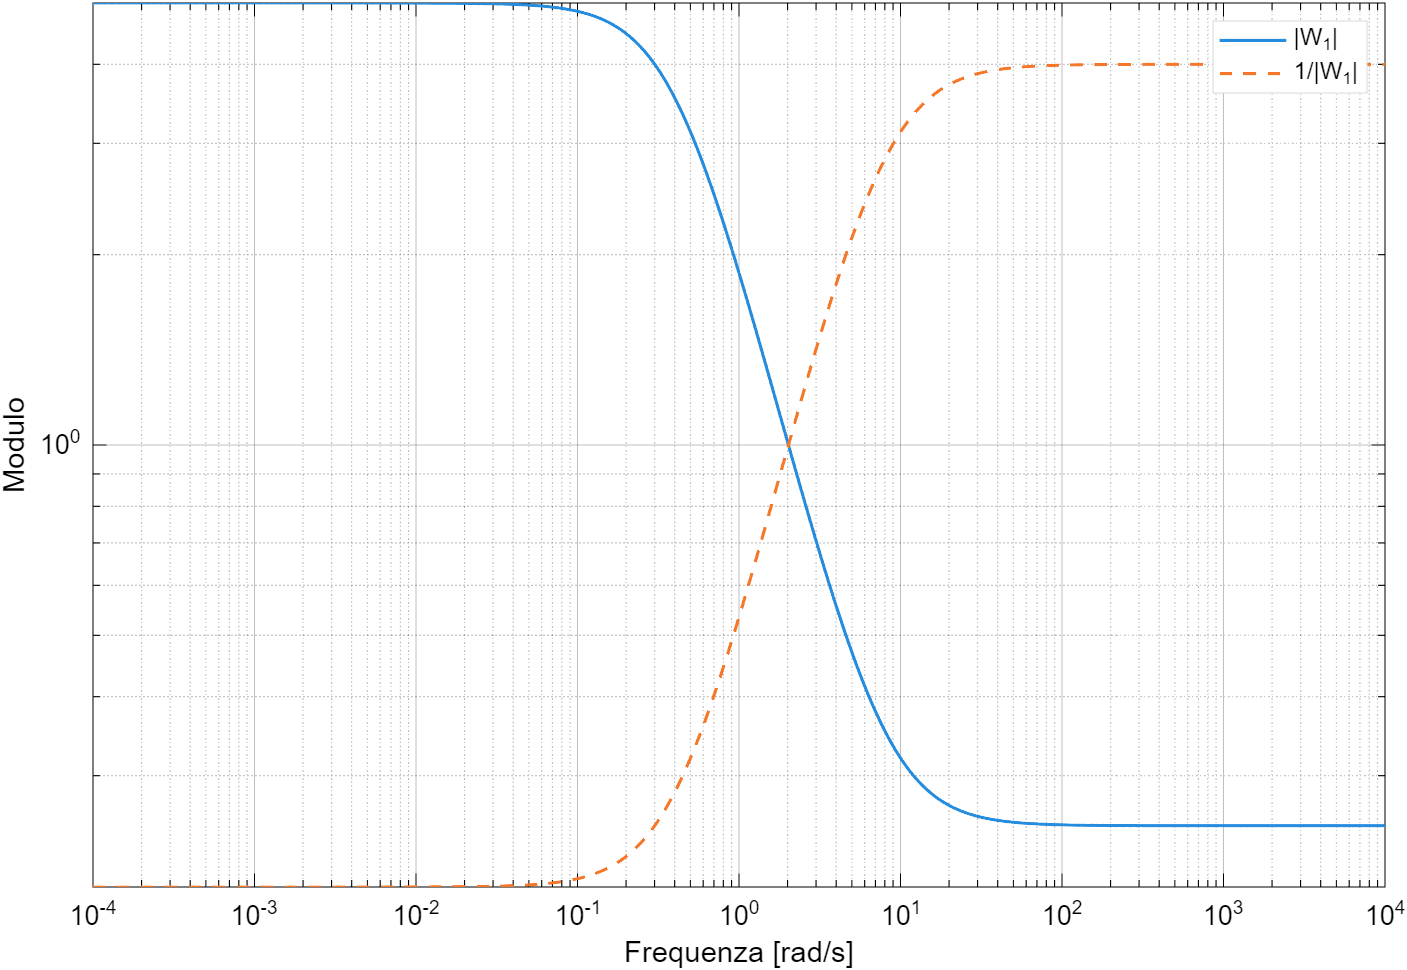
\includegraphics[width=0.86\textwidth]{figures/hinf_targeted_revision/01_W1.png}
\caption{Peso W1 e inverso: accuratezza e rilassamento in frequenza.}\end{figure}
\begin{figure}[p]\centering
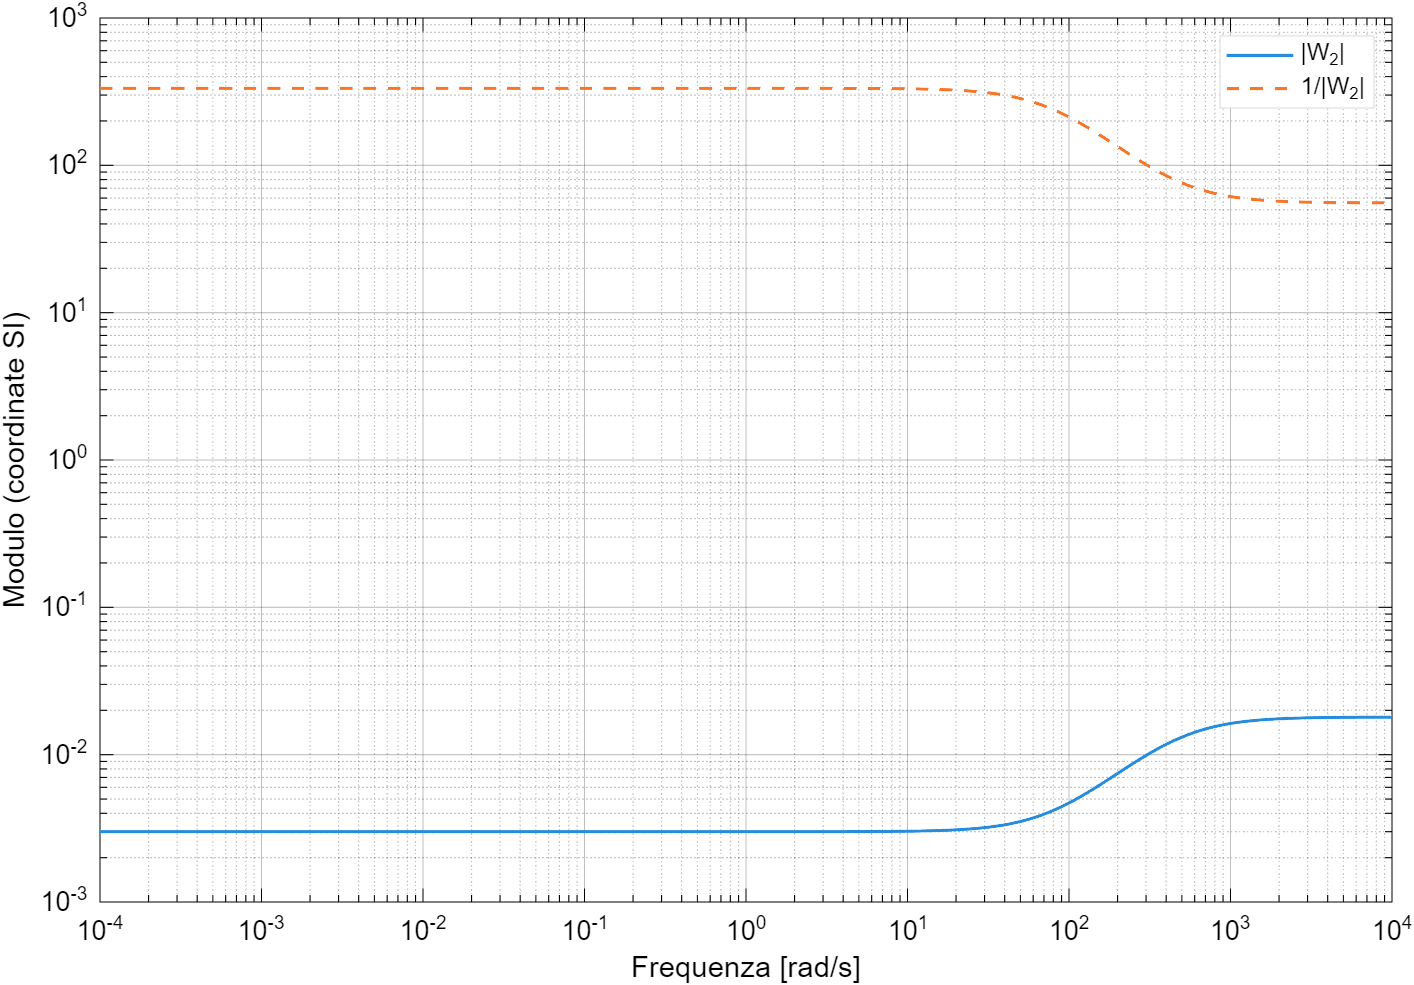
\includegraphics[width=0.86\textwidth]{figures/hinf_targeted_revision/02_W2.png}
\caption{Peso W2 e inverso: penalizzazione del comando nelle coordinate SI.}\end{figure}
\begin{figure}[p]\centering
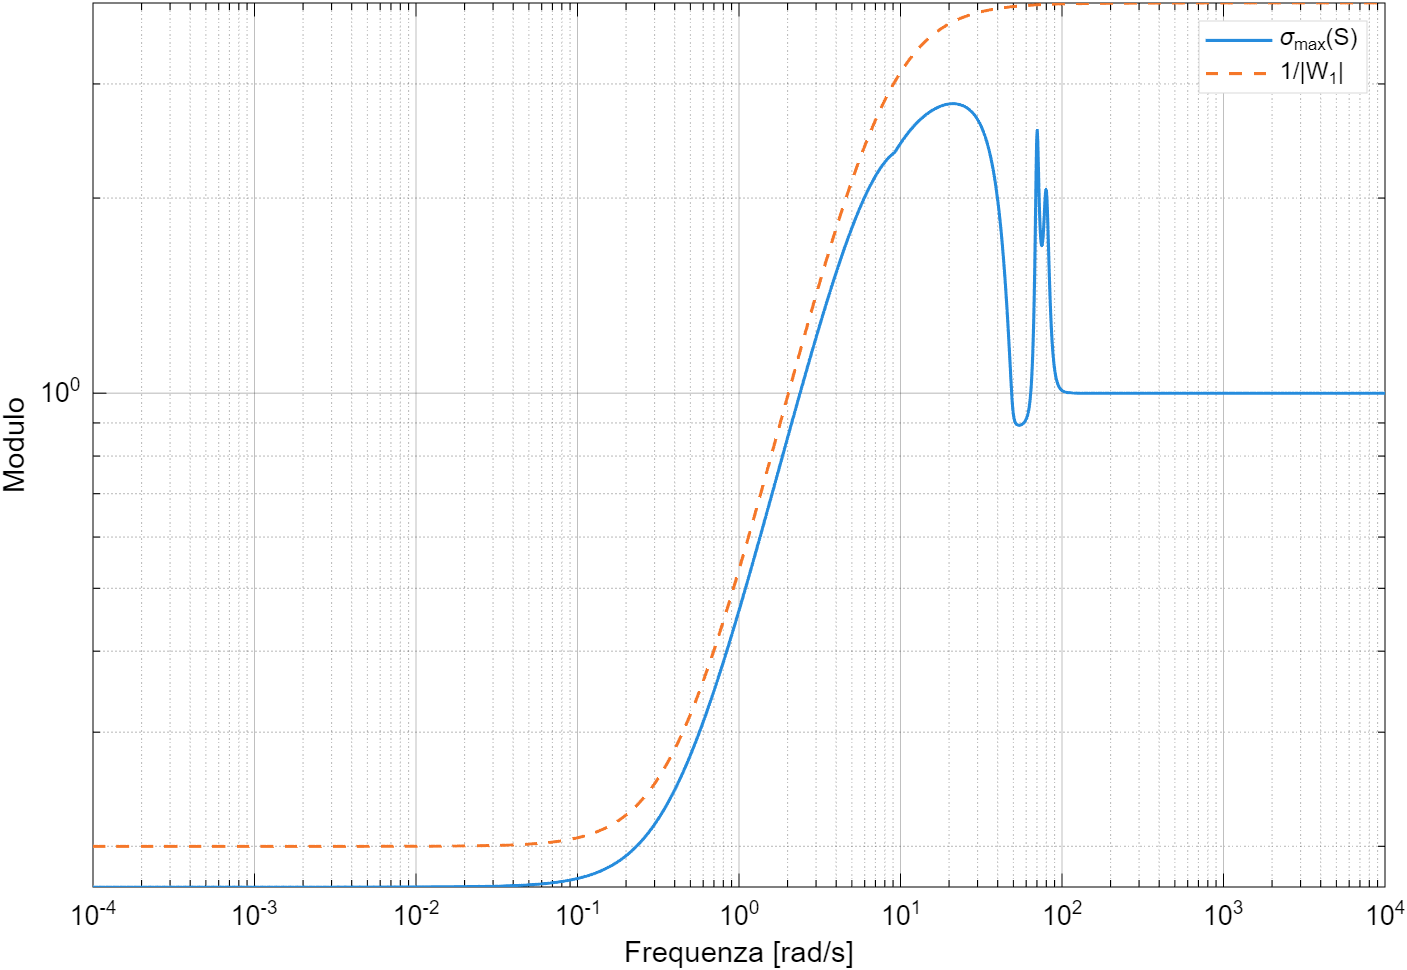
\includegraphics[width=0.86\textwidth]{figures/hinf_targeted_revision/03_S.png}
\caption{Sensitivity rispetto al nuovo inviluppo.}\end{figure}
\begin{figure}[p]\centering
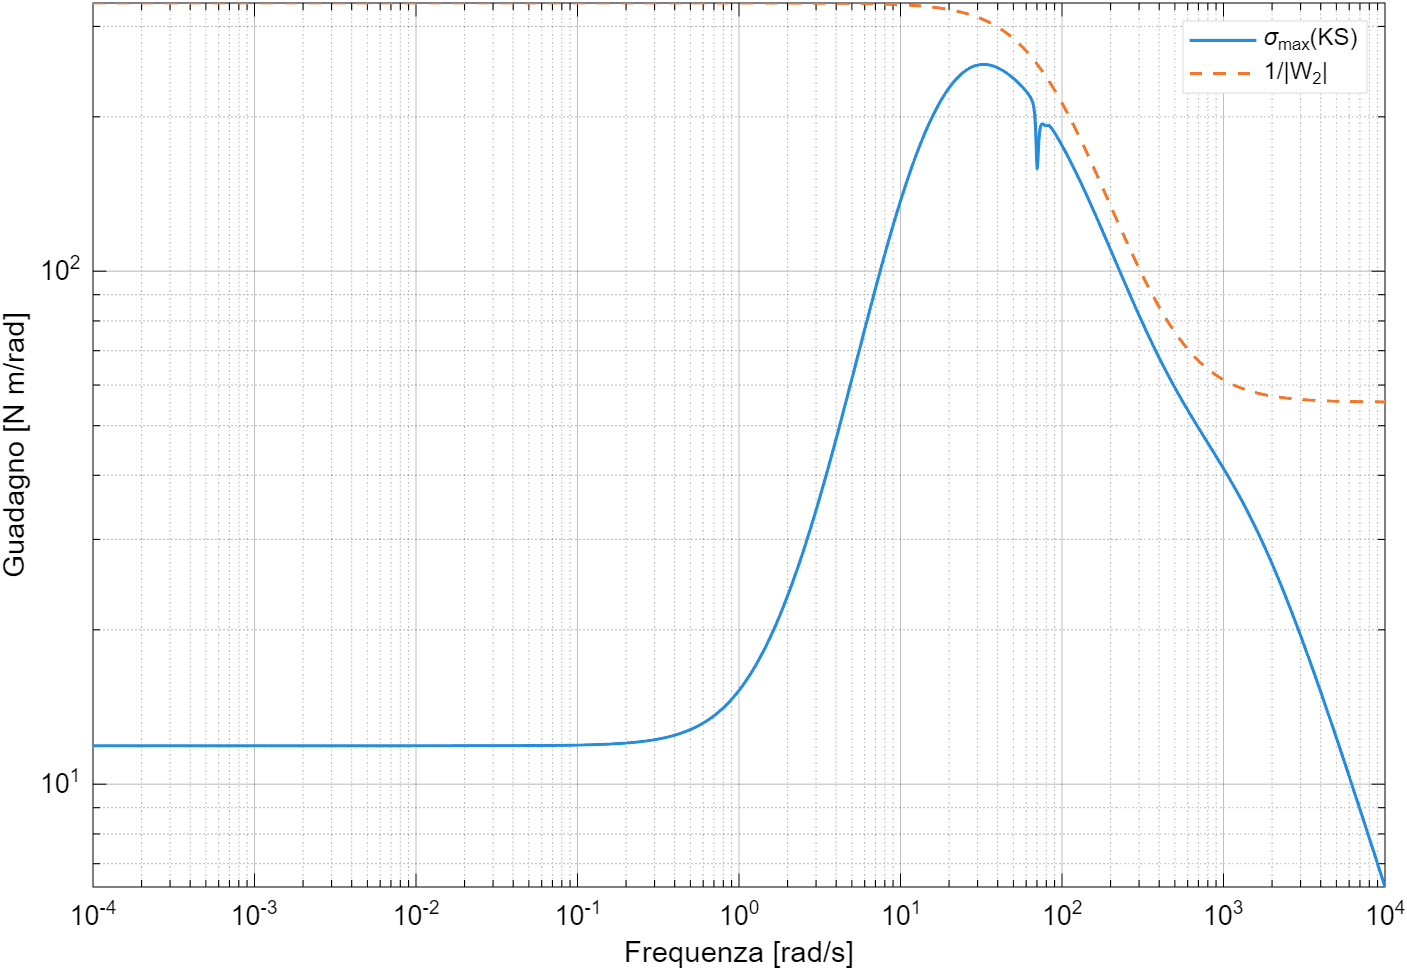
\includegraphics[width=0.86\textwidth]{figures/hinf_targeted_revision/04_KS.png}
\caption{Mappa del comando rispetto al nuovo inviluppo.}\end{figure}
\begin{figure}[p]\centering
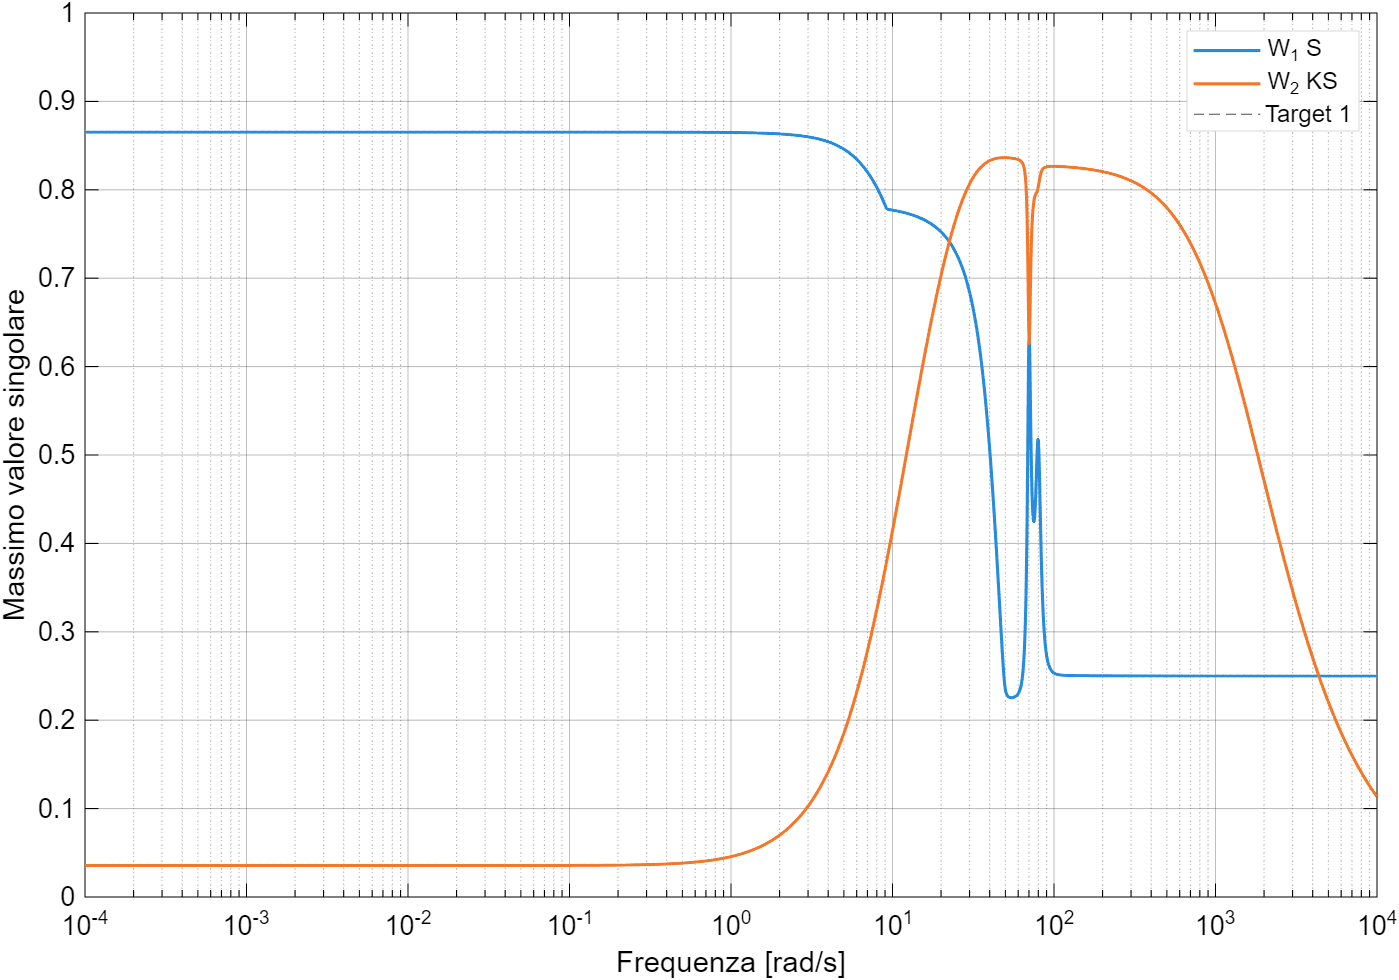
\includegraphics[width=0.86\textwidth]{figures/hinf_targeted_revision/05_weighted.png}
\caption{Canali pesati e livello uno.}\end{figure}
\begin{figure}[p]\centering
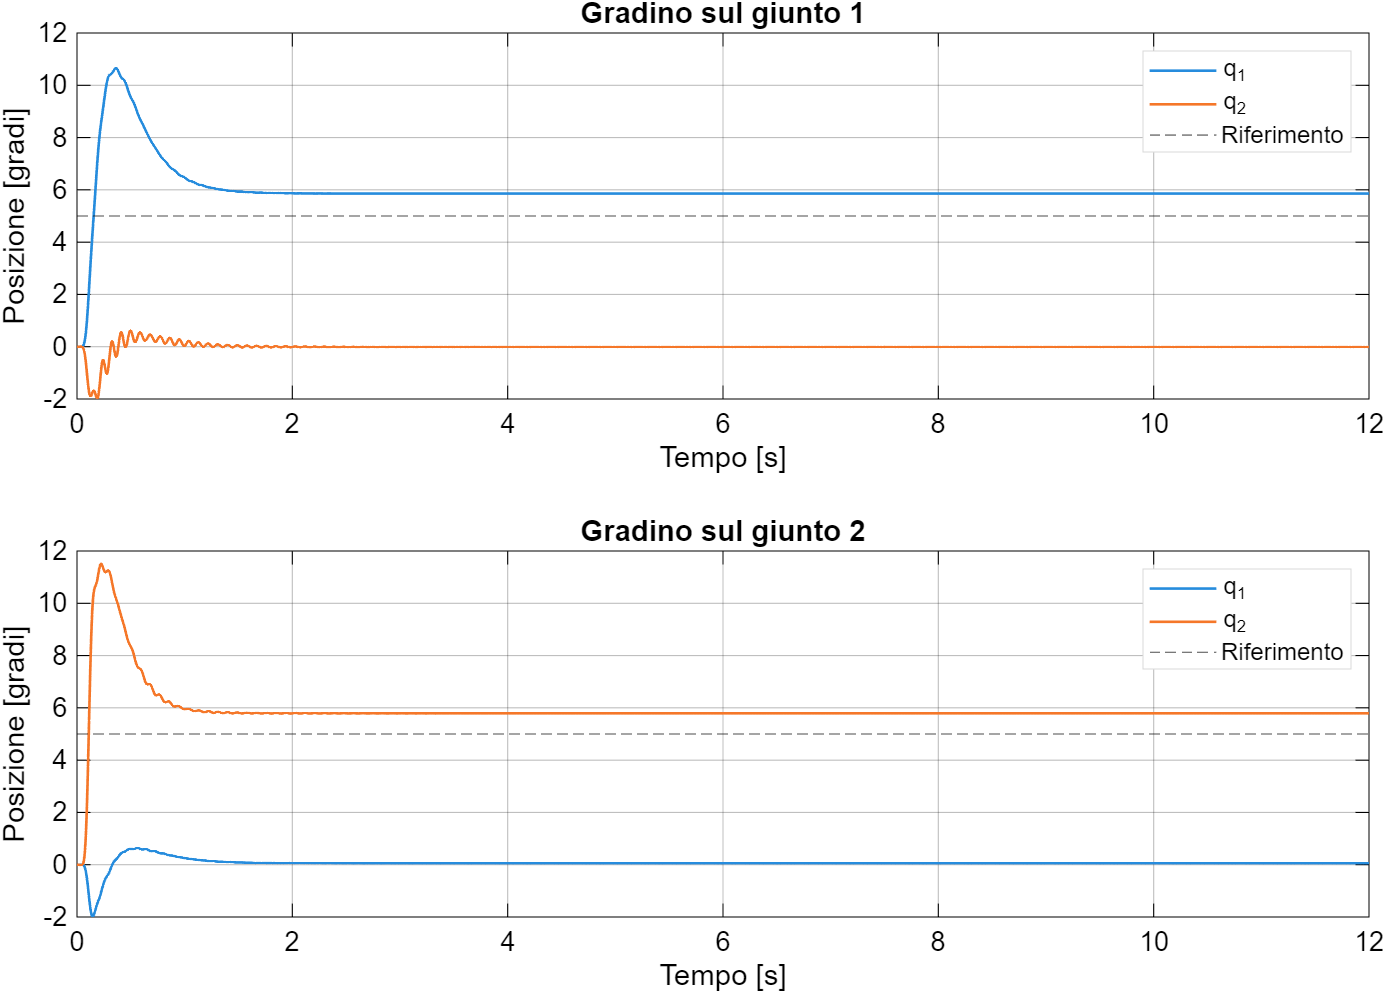
\includegraphics[width=0.86\textwidth]{figures/hinf_targeted_revision/06_tracking.png}
\caption{Due gradini separati da 5 gradi: il PASS pesato non elimina l'overshoot.}\end{figure}
\begin{figure}[p]\centering
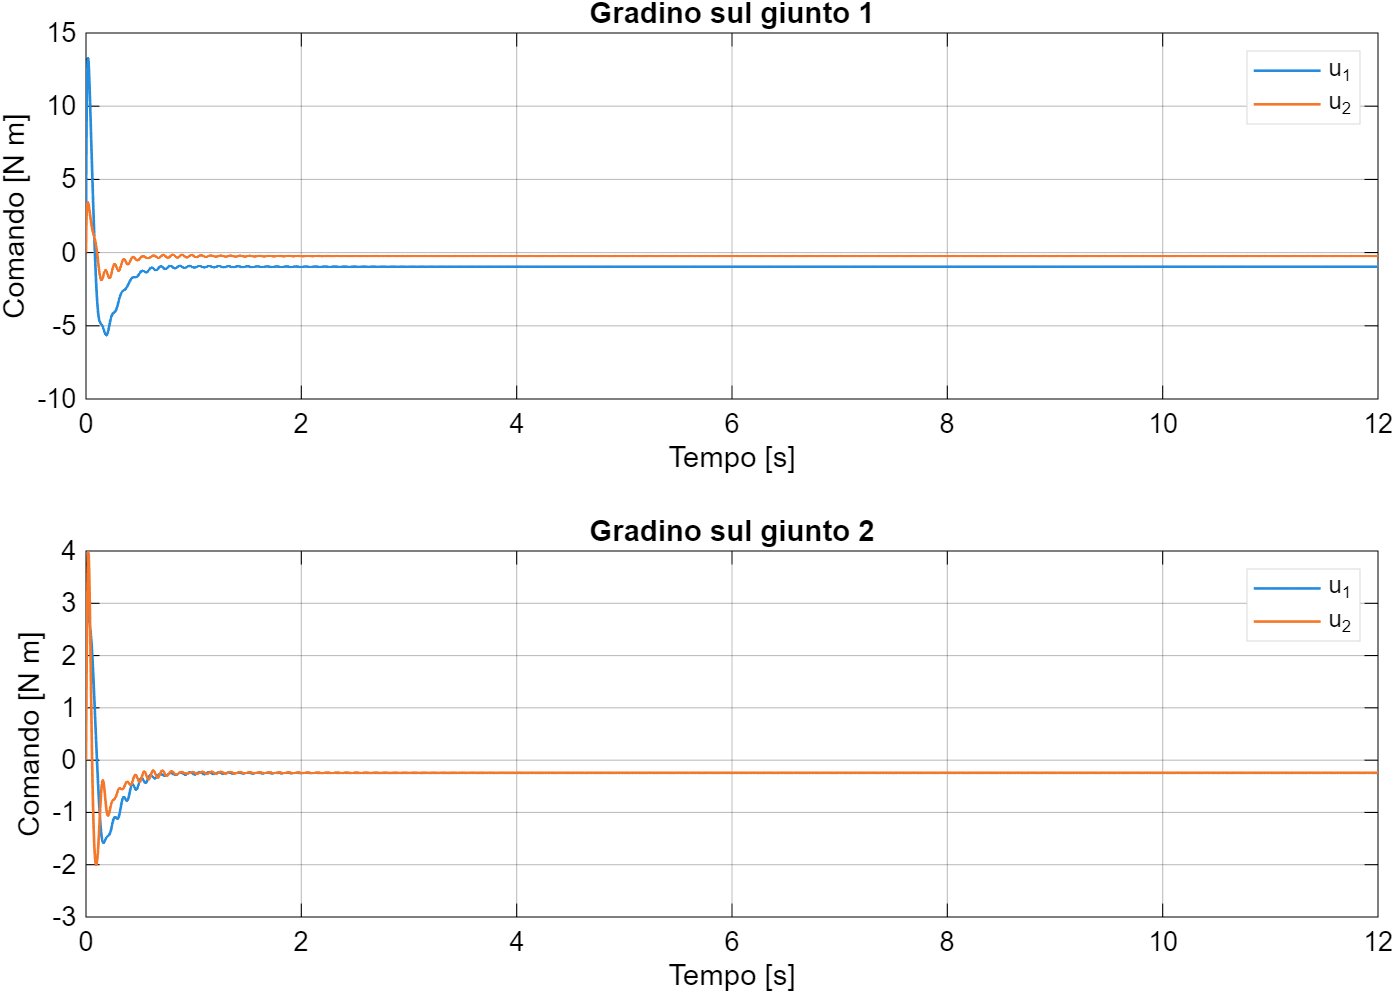
\includegraphics[width=0.86\textwidth]{figures/hinf_targeted_revision/07_control.png}
\caption{Coppie richieste nei medesimi esperimenti.}\end{figure}
\begin{figure}[p]\centering
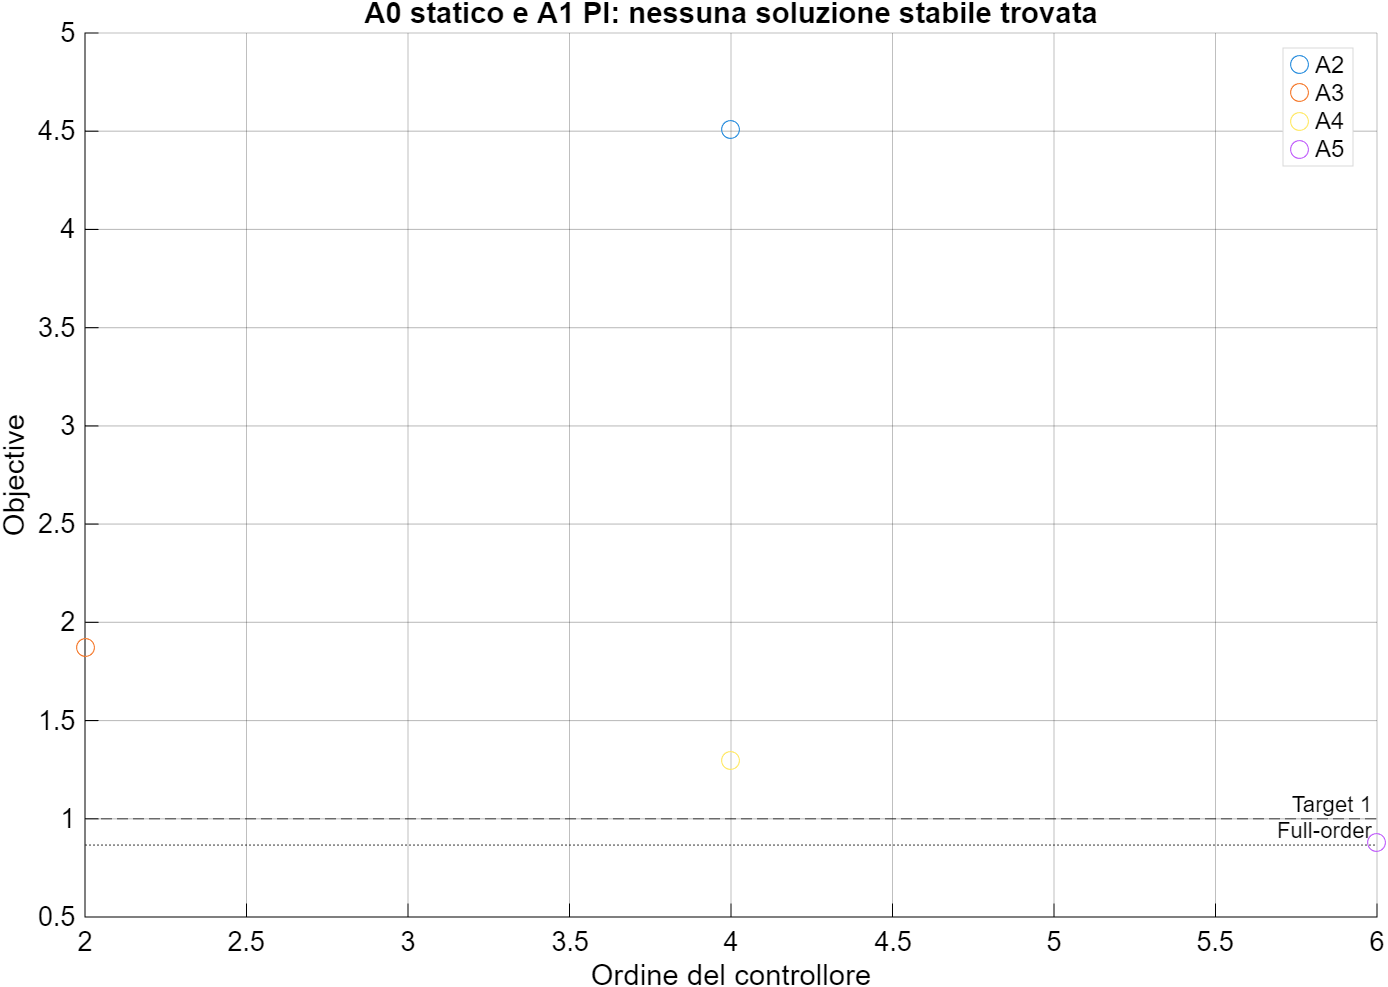
\includegraphics[width=0.86\textwidth]{figures/hinf_targeted_revision/08_fixed_order.png}
\caption{Frontiera ordine--objective; vengono conservati gli esiti negativi.}\end{figure}
\begin{figure}[p]\centering
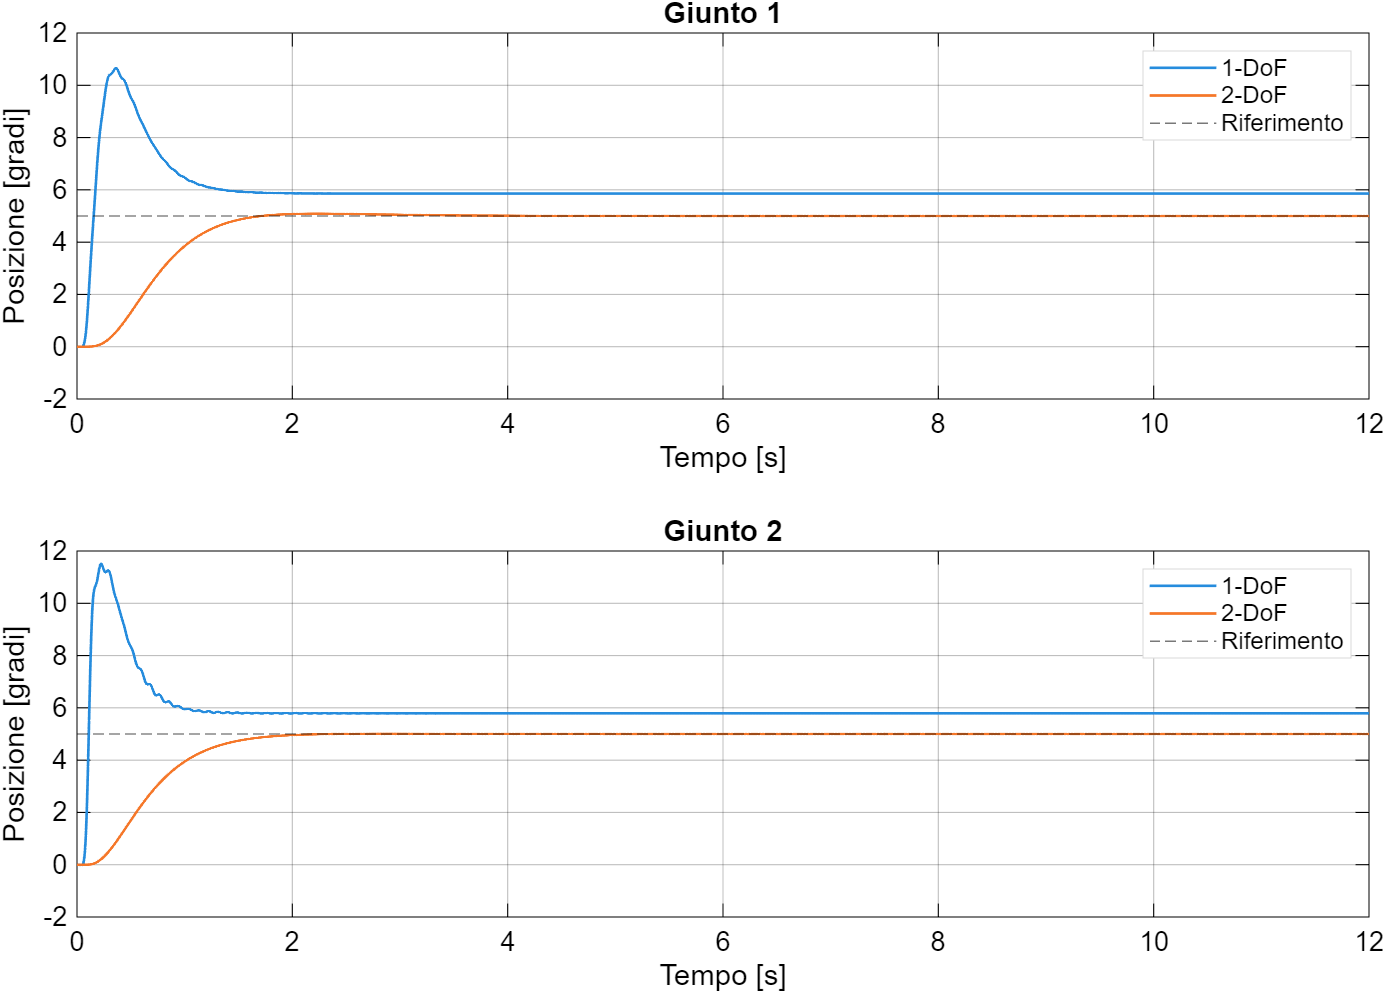
\includegraphics[width=0.86\textwidth]{figures/hinf_targeted_revision/09_2dof.png}
\caption{Confronto 1-DoF/2-DoF sulla stessa pianta e sugli stessi riferimenti.}\end{figure}
\begin{figure}[p]\centering
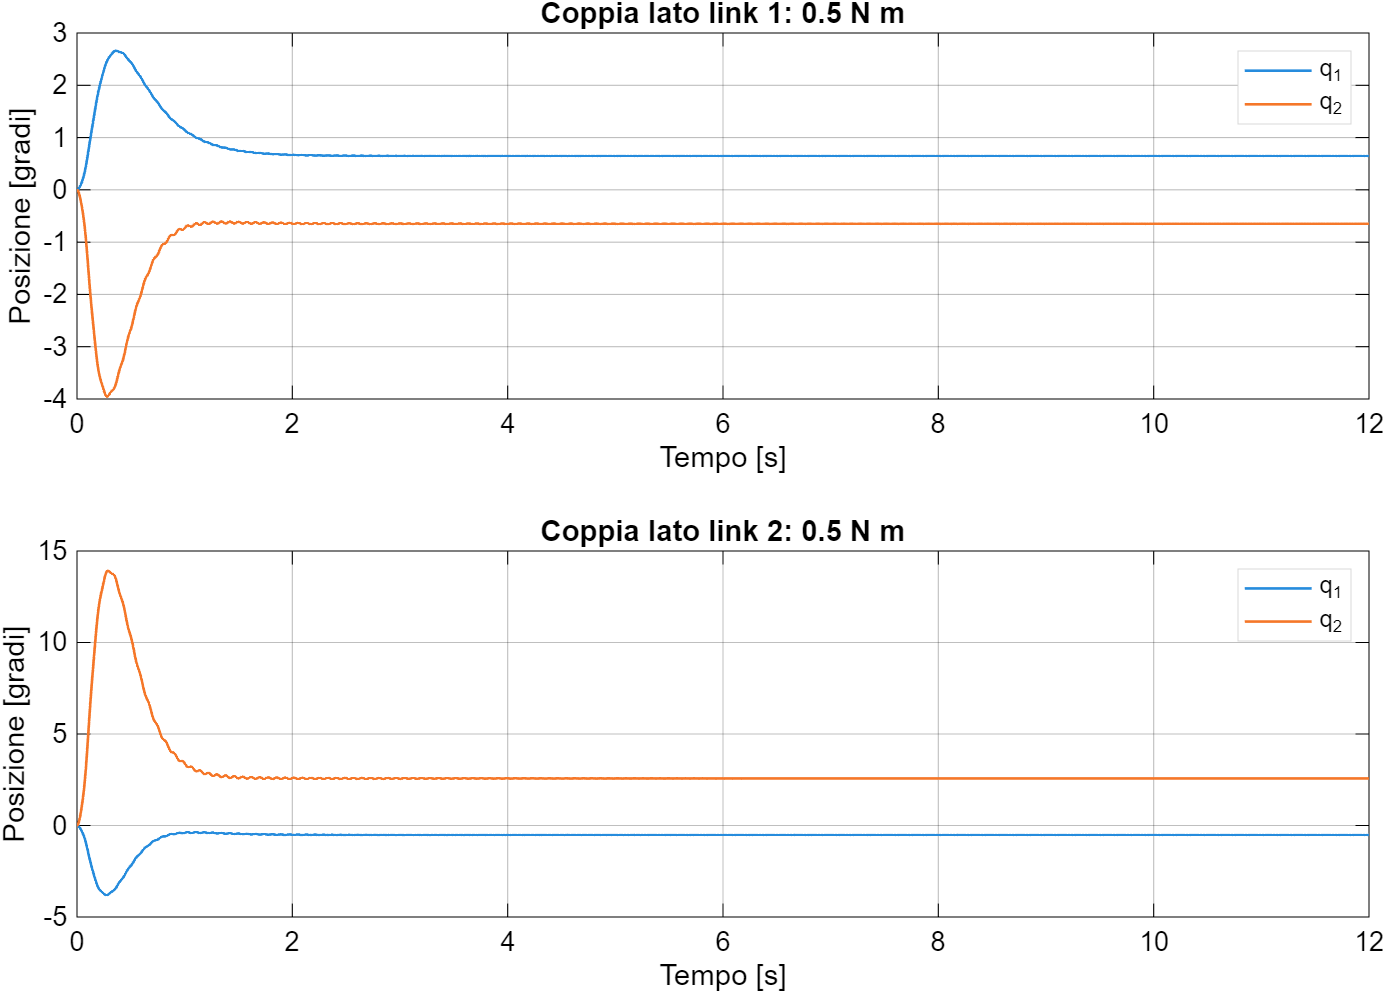
\includegraphics[width=0.86\textwidth]{figures/hinf_targeted_revision/10_link_disturbance.png}
\caption{Verifica fisica con coppie disturbanti lato link di 0.5 N m.}\end{figure}

Gli script dedicati \path{run_hinf_revision},
\path{run_hinf_revision_fixed}, \path{extend_hinf_revision_2dof}
ed \path{export_hinf_revision} leggono M3/M5 congelati e scrivono
soltanto i nuovi artifact. I checkpoint evitano di ripetere sintesi
gia' eseguite. Il comando generale \texttt{run\_all} rimane riferito
alla pipeline storica e non e' stato eseguito in questa revisione.
I sette test mirati verificano identita', stabilita' interna, bound,
66 avvii, metriche e separazione dei criteri. La valutazione e' nominale
lineare: nessuna RAS o garanzia robusta viene trasferita ai nuovi K.
La revisione si arresta qui: nessuna nuova $\mu$-analysis o $\mu$-synthesis.
\clearpage
